
\chapter
{The PEBL Launcher}

The PEBL Launcher is the best way to navigate and launch PEBL
experiments, especially for novices or research assistants.  It allows
one to specify a few specific options that are frequently changed,
navigate through the PEBL Test Battery, and create and save
'experiment chains' to let you run multiple experiments in a row.

\begin{figure}[h]
\caption{Screenshot of of PEBL Launcher.}
\center
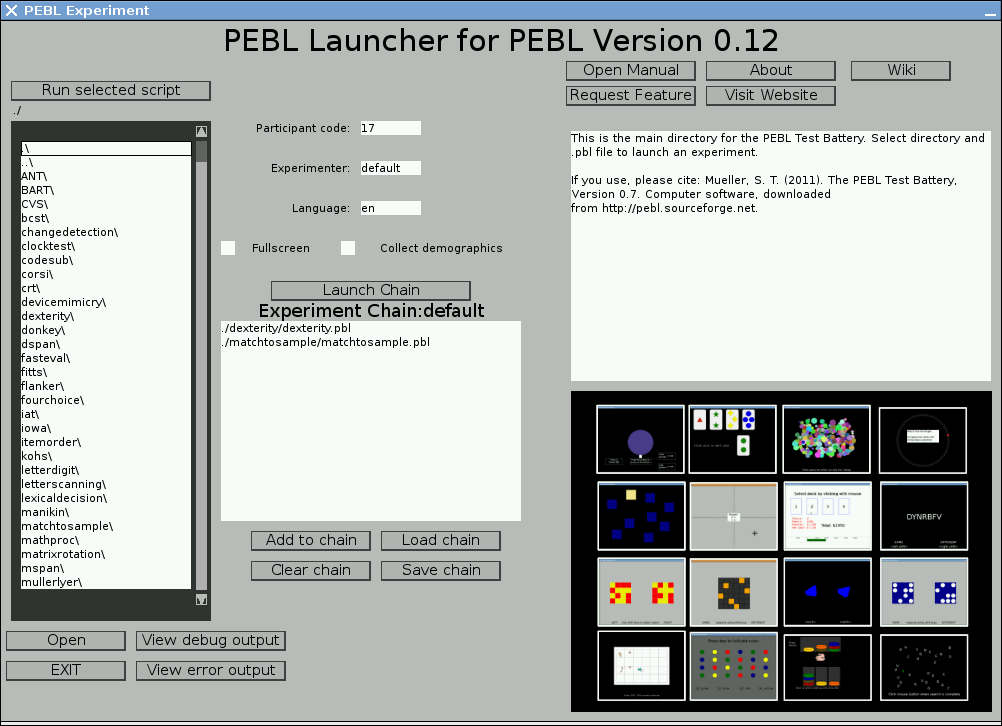
\includegraphics[scale=.35]{launcher.png} 
\end{figure}
\clearpage
\sect{History of the Launcher}
Prior to 2011, a front-end launcher was only available for PEBL on
Windows.  It was written in Visual Basic 6, which was old-fashioned,
single-platform, no longer supported by Microsoft, and created a
situation where a critical piece of PEBL infrastructure depended on a
non-free tool.  The main obstacle to a new launcher has always been:
PEBL needs a cross-platform launcher using a free software, and we
don't want to have to distribute a whole additional interpreter.  This
means that Python, wxBasic, TCL/TK, etc. were out of the
consideration.  Why couldn't there be an easy-to-use cross-platform
programming tool we could use?

As of PEBL Version 0.12, we found one: PEBL itself.  PEBL is not
really designed to create GUI applications, but it can be beat into
submission to do so.  For Version 0.12, enough filesystem access
functions and other features were available to make a reasonable
launcher.  Although the old-style launcher will probably still work,
it will no longer be supported.  The new launcher will not integrate
completely seamlessly into your operating system, but it is designed
to support the important functions of setting up and launching an
experiment.

\sect{How it works}
The simplest usage of the Launcher is that you use the file selector on
the left to choose a .pbl file, then click the button 'Run selected
script'' to run that experiment.  ONLY .pbl files and directories will
appear in the file window.
\clearpage
\sect{Features}

\begin{wrapfigure}{r}{0.5\textwidth}
 \vspace{-40pt}
  \begin{center}
    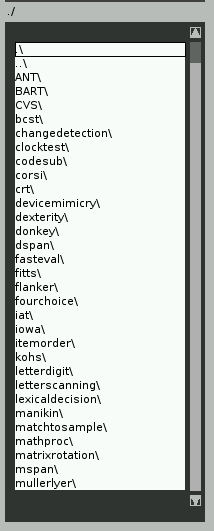
\includegraphics[scale=.5]{filebrowser.png} 
  \end{center}
  \caption{The PEBL Launcher File Browser.}
 \vspace{-50pt}
\end{wrapfigure}
\subsection{File browser}
On the left is a file browser.  It will only show .pbl files and
subdirectories.  To navigate to a subdirectory, simply click on the
directory to select it, then click on the selected directory.  To move
back up a directory, click on the '..\textbackslash' row.  When you have a .pbl file
selected, you can use the 'Run selected script' button to launch it.


\subsection{Participant code}
This will allow you to select the participant code you want sent to
any experiments you are about to run.  By default, PEBL saves the last
experiment code when you exit, and then reloads it the next time,
incrementing by one.  This makes it easier to avoid colliding
participant codes and overwriting data.  Participant code need not be
a number, but the launcher currently does not understand how to
increment non-numeric codes, and will probably restart at 1.  The plus button next to the 
code box will increment the current number by 1, which is useful if you are running multiple sessions in a row.

The automatic incrementation of participant code can be turned off by
opening the fileselect.pbl file and changing the variable gAutoSubcode
from 1 to 0.

When an experiment is launched, the specified code will be fed into
the experiment using the -s command-line option, and will be bound to
the gSubNum variable.  Some of the standard experiments will ask you
to enter a participant code regardless of whether you have one selected.
If that is the case, you should be able to edit the script to remove
the request to specify a participant code. However, most experiments in
the test battery should only ask the experimenter to specify a participant
code if the participant code is '0', which is what it will be when no -s
command is given.  So, if you are using code 0, many of the
experiments will ask you to enter a code after they launch.


\subsection{Experimenter code}
Many times, you may wish to keep track of the experimenter or research
assistant who collected the data.  Have them enter their name in the
'experimenter' window.  The name will be saved on exit.  The
experimenter code will be saved to the runlog file (see below). 

\subsection{Language}
Some experiments have instructions and stimuli that are translated
into different languages.  Enter your two-character language code in
the language box to tell the experiment what language to use. If your
chosen language is not available, the experiment will fall back to
English.  If you want to translate an experiment into your own
language, ask on the PEBL mailing list.

\subsection{Fullscreen Mode}
If you want to launch your experiment in full-screen mode to improve
video latency and to avoid distractions, check this box. The secret
escape key combo is ctrl-alt-shift-\textbackslash : hit these four to abort out of
an experiment before it is complete.

\subsection{Demographics Collection}
The U.S. NIMH requires a number of demographic variables for research
they fund. Checking this box will collect this data and save it to a
data log file called demographics-log.csv, prior to running your experiment or experiment chain.

\subsection{Experiment Chains}
The launcher allows you to set up a 'chain' of experiments that get run in sequence.  All the experiments will be run consecutively, with an identical subject code.  This is accomplished by running a separate instance of PEBL for each experiment.  The different experiments have no ability to communicate directly with one another.


\subsection{Saving Experiment Chains}
When you exit the launcher, the current experiment chain will get saved in the the current config file.  By default, this file is called default.config.  This same file is loaded when the launcher starts again, restoring your settings.  In addition, a chain can be saved with a different name, and loaded, either at start-up (by specifying the name of the config file with the -v command-line option), or by entering the name in the dialog that occurs when 'Load  Chain' is clicked.

\subsection{Loading Experiment Chains}
A previously saved experiment chain can be loaded using the 'load chain' button.  If a config file with that name exists, it will load the settings and the experiment chain in that file.  If no file exists with the specified name, it will change the name from 'default' (or whatever the current chain is called) to the specified name, and save the current configuration to the new configuration file on exit or when the 'save chain' button is clicked.

\subsection{Description and Screenshot}
On the right side of the launcher is a window that will show a screenshot and print a description of a script when it is highlighted.  These need to be created by hand for each script.


\subsection{Commmand Line Options}
There are a number of command line options available for PEBL that are not present as options in the launcher.  If you want to use any, you can type them in the ``Command line Options'' box and the launcher will pass them to PEBL.  You can use these to specify -V options that pass parameters into your experiment (e.g., controlling whether a practice or a test round is given).

\subsection{Other buttons}
The launcher has a number of other buttons to help you use PEBL.
These include:
\begin{itemize}

\item \emph{Open} On the lower left, there is a button labeled ``Open''.  This
  will open a selected .pbl script in a text editor, and will open a
  directory in your system's file manager.  An easy way to look at or
  make changes to the script, or to locate data files after a script is run. 

\item \emph{View debug output} Whenever an experiment is run, any time
  you use the Print() function, it will print the resulting text to a
  file names stdout.txt the directory it was run in.  This button will
  open that file.

\item \emph{View error output} Whenever an experiment is run, the
  error and status messages are saved to a file called stderr.txt in
  the directory it was run in.  This button will open that file.

\item \emph{Exit} This will exit the launcher and save the current
  configuration options to the named experiment chain.

\item \emph{Open manual} This opens the PEBL .pdf manual.  The manual
  is located in different places on each platform, and will change
  names for each release.

\item \emph{About} This provides a short description of the launcher.

\item \emph{Visit Website}  This will take you to the main PEBL website.

\item \emph{Request Feature}  This takes you to the PEBL Fundry
  website, where you are able to request a feature (including new
  experiment scripts).  Fundry allows you to pledge a donation for
  your feature, allowing you to support PEBL and be a driver
  of its development.

\item \emph{Wiki} This button will take you to the PEBL wiki, and do
  its best to find a WIKI page related to the experiment you are
  looking at. They won't always exist, and if not, you can always sign
  in and make your own.

\end{itemize}

\sect{Launching an experiment}

To launch an experiment, navigate through the directories in the file listing box.  Only directories and files with the .pbl extension are shown in this box.  To open a directory, click once to move the highlight box onto the directory name, and a second time to open the directory.  When a new directory is opened, the first available .pbl file will be automatically selected.  To run that script, just press the 'Run Selected script' button above the file select box.  It will run with the specified parameter, including subject code, language, fullscreen mode.  In addition, if the 'collect demographics' button is selected, a demographic survey will happen prior to the study running.

\sect{Launching an experiment chain}
If you have a series of experiments you want to run, create an experiment chain and launch it using the 'Launch chain' button above the experiment chain selection box.  Tip: Use experiment chains even if you are are running just single experiment, with just a single experiment selected.  This give faster access and is less error-proned.

\sect{Translating the Launcher}
You can translate the launcher to your own language.  Open the launcher file (fileselect.pbl), and go to the end of the script, to a function named "GetStrings":
\begin{verbatim}
define GetStrings(lang)
{
   lang <- Uppercase(lang)
   if(lang == "EN")
   {
      gRunText <- "Run selected script"
      gOpenText <- "Open"
      gExitText <- "EXIT"
      gViewDebugText <- "View debug output"
      gViewErrorText <- "View error output"
      gAddToChainText <- "Add to Chain"
      gClearChainText <- "Clear Chain"
      gSaveChainText <- "Save Chain"
....
\end{verbatim}

The labels used in the launcher all appear here.  You should be able to just translate the text of each on into the language of your choice.  Send the translations back to the author so they can be incorporated into the next launcher version.  You can also make a section in the if statement for your particular language.  When you change the language in launcher, it will save that option and use your language of choice next time.

%%% Local Variables: 
%%% mode: latex
%%% TeX-master: "main"
%%% End: 
